\section{Applications}

\begin{frame} {Short-lived Radioisotopes (SLRs) Production}
    \begin{itemize}
        \item SLRs: such as $^{13}$N, $^{17}$F, $^{18}$F, $^{15}$O, and $^{11}$C.
        \item SLRs are used in medical applications.
        \item SLRs production: bombardment of an external solid (exogenous method).
        \item SLRs production: bombardment of a high atomic number gas (endogenous method).
    \end{itemize}
    \begin{figure}
        \centering
        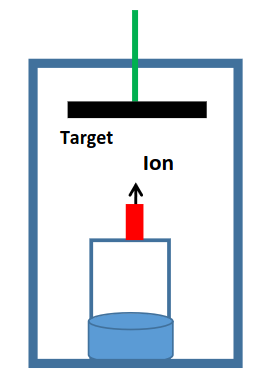
\includegraphics[width=0.2\textwidth]{figures/slr-production.png}
        \caption{The bombardment of target by ion beam generated by plasma.}
        \label{fig:slr-production}
    \end{figure}
\end{frame}

\begin{frame} {Thin Film Deposition}
    \begin{itemize}
        \item Thin film deposition: create thin film coating onto a substrate material.
        \item Electron beam sputters target material.
        \item Sputtered material gets deposited onto the surface of substrate material.
    \end{itemize}
    \begin{figure}
        \centering
        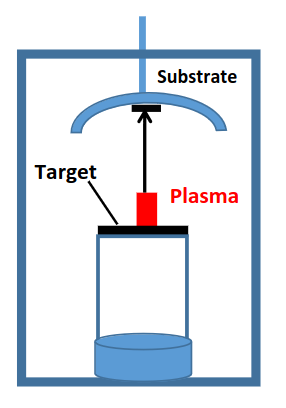
\includegraphics[width=0.2\textwidth]{figures/thin-film-doposition.png}
        \caption{Schematic arrangement for thin film deposition in a plasma focus.}
        \label{fig:thin-film-deposition}
    \end{figure}
\end{frame}

\begin{frame} {Detection of Illicit Materials and Explosives}
    \begin{itemize}
        \item The neutron scattering and the gamma-rays allows us to determine the material.
        \item DFP is a good neutron source.
    \end{itemize}
    \begin{figure}
        \centering
        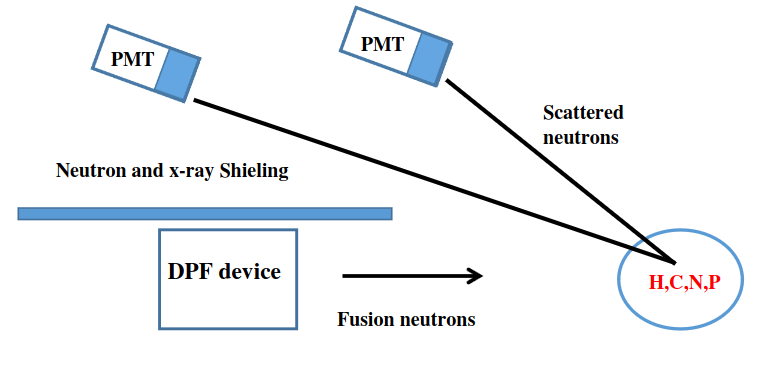
\includegraphics[width=0.7\textwidth]{figures/detection-of-illicit-material.png}
        \caption{Schematic arrangement of illicit and explosive materials detection by a DPF.}
        \label{fig:detection-of-illicit-material}
    \end{figure}
\end{frame}